\documentclass[a4paper]{amsart}

\usepackage{color}
\usepackage[colorlinks=true, citecolor=red]{hyperref}  %needs to come before amsrefs package to work with
 \usepackage{amssymb,latexsym}
\usepackage[alphabetic]{amsrefs}
\usepackage[mathscr]{eucal}
\usepackage{pdfsync}
\usepackage{graphicx}
\usepackage{epstopdf}
\DeclareGraphicsRule{.tif}{png}{.png}{`convert #1 `dirname #1`/`basename #1 .tif`.png}
\usepackage[all]{xy}
\usepackage{titletoc}

\CompileMatrices

\theoremstyle{plain}
\newtheorem{theorem}{Theorem}[section]
\newtheorem{lemma}[theorem]{Lemma}
\newtheorem{proposition}[theorem]{Proposition}
\newtheorem{corollary}[theorem]{Corollary}

\theoremstyle{definition}
\newtheorem{definition}[theorem]{Definition}%[section]

\theoremstyle{remark}
\newtheorem{example}[theorem]{Example}
\newtheorem{remark}[theorem]{Remark}
\newtheorem{discussion}[theorem]{Discussion}
\DeclareMathOperator{\Lip}{Lip}
\DeclareMathOperator{\dist}{dist}
\DeclareMathOperator{\expected}{\mathbb{E}}
\DeclareMathOperator{\prb}{Prob}
\DeclareMathOperator{\spt}{spt}
\DeclareMathOperator{\lap}{\Delta}

\raggedbottom

\addtolength{\textwidth}{2cm}
\addtolength{\oddsidemargin}{-1cm}
\addtolength{\evensidemargin}{-1cm} 
\addtolength{\topmargin}{-1cm} 
\addtolength{\textheight}{2cm}
% \renewcommand{\l@subsection}{\@contentsline{2}{5em}{7em}}

%\makeatletter
%\makeatother

 
%%% BEGIN DOCUMENT
\begin{document}

\title{Diffusion on SG(2)}  
\author{John E.\ Hutchinson}
\date{\today}

\maketitle


%\renewcommand*\l@subsection{\@tocline{4}{50em}{7em}{10em}{10em}}


\tableofcontents

I follow mainly \cite{Bar1}*{Section 2}.

%%%%%%%%%%%%%%%%%%%%%%%%%%%%%%%%%%%%%%
%%%%%%%%%%%%%%%%%%%%%%%%%%%%%%%%%%%%%%%%
%%%%%%%%%%%%%%%%%%%%%%%%%%%%%%%%%%%%%%%%%%
\section{\textbf{Notation}}

\begin{figure}[htbp] %  figure placement: here, top, bottom, or page
   \centering
   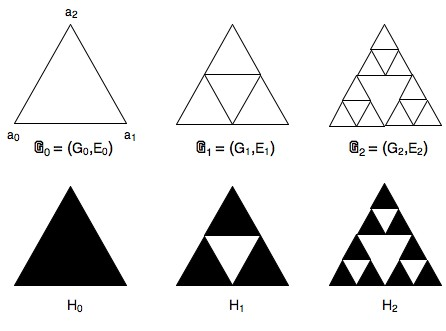
\includegraphics[width=4in]{prefrac.jpg} 
   \caption{SG(2) approximating graphs and sets.}
   \label{prefrac}
\end{figure}

$ H_0 $ is  the closed convex unit triangle in $ \mathbb{R}^2 $.
$ G_0 = \{a_1,a_2,a_3\}   $ is the set of vertices.

$ H_n $ is the union of $ 3^n $ scaled copies of $ H_0 $, each of side $ 2^{-n} $.
$ G_n $ is the set of vertices of $ H_n $.

$ E_n $ is the set of edges.  
$ \mathbb{G}_n := (G_n, E_n) $ is the corresponding graph.

\medskip $ G = SG(2) := \bigcap_{n\geq 0} H_n $.

\medskip
An \emph{$ n $-triangle} is any one of the $ 3^n $ triangles in $ H_n $.

An \emph{$ n $-complex} is a set of the form $ G \cap B $ where $ B $ is  an  $ n $-triangle.

$ \mathcal{S}_n $ is the set of $ 3^n $ $ n $-complexes.

For $ x \in G_n $, $ D_n(x) =  \bigcup \{ S\in \mathcal{S}_n : x \in S \} $.  (So unless $ x \in \{ a_0,a_1,a_2\} $, there are exactly two sets in this union.)

%%%%%%%%%%%%%%%%%%%%%%%%%%%%%%%%%%%%%%%%%%%%%%%
%%%%%%%%%%%%%%%%%%%%%%%%%%%%%%%%%%%%%%%%%%%%%%%%%%
%%%%%%%%%%%%%%%%%%%%%%%%%%%%%%%%%%%%%%%%%%%%%%%
\section{\textbf{Flat Measure}}
Define $ \mu_n $ to be Lebesgue measure restricted to $ H_n $, normalised so $ \mu_n(H_n) = 1 $.

Define the \emph{flat measure} on $ G $ by $ \mu_G := \text{weak lim}_{n\to\infty} \mu_n $.  It assigns mass $ 3^{-n} $ to each $ n $-cell.

Define the \emph{fractal  dimension} $ d_f := \log 3 / \log 2 $.   It is the scaling dimension   for fractals generated by similitudes and satisfying the open set condition.  It is also the Hausdorff dimension.

\medskip
It follows (easy) for $ x \in G $ and $ 0\leq r <1$ that
\[   3^{-1} r^{d_f}   \leq \mu_G B_r(x) \leq 18  r^{d_f}.\]
(The   constants  3 and 18 are unimportant.)

%%%%%%%%%%%%%%%%%%%%%%%%%%%%%%%%%%%%%%%%%%%%%%%
%%%%%%%%%%%%%%%%%%%%%%%%%%%%%%%%%%%%%%%%%%%%%%%%%%
%%%%%%%%%%%%%%%%%%%%%%%%%%%%%%%%%%%%%%%%%%%%%%%
\section{\textbf{Geodesic Metric}}
For any \emph{closed} $ A \subset \mathbb{R}^d  $ and $ x,y \in   A $ define 
\begin{equation} \label{}
d_A (x,y) = \inf \{ |\gamma | : \gamma \text{ is a path between $ x $ and $ y $ with }   \gamma \subset A \}.
\end{equation}

\emph{If $ d_A $ is finite for all $ x,y \in A $ then $ d_A $ is a metric.}  It is  called the \emph{geodesic metric} on $ A $. 
In this case, $ (A,d_A) $ satisfies the geodesic property:  

\emph{For each $ x,y \in  A $ there exists  a map $ \Phi:[0,1] \to A $ such that} 
\[  d_A(x,\Phi(t) ) = t d_A(x,y), \quad d_A(\Phi(t),y ) = (1-t )d_A(x,y), \quad \forall t \in [0,1]  .\]
\emph{Proof}:  Take a   sequence of approximating maps and use a diagonal argument.

\medskip For $ G $ one obtains
\begin{equation} \label{}
|x-y| \leq d_G(x,y) \leq 8 |x-y|.
\end{equation} 
\emph{Proof}: By a chaining argument.

(As usual, the constants 1 and 8 are unimportant.) 
%%%%%%%%%%%%%%%%%%%%%%%%%%%%%%%%%%%%%%%%%%%%%%%
%%%%%%%%%%%%%%%%%%%%%%%%%%%%%%%%%%%%%%%%%%%%%%%%%%
%%%%%%%%%%%%%%%%%%%%%%%%%%%%%%%%%%%%%%%%%%%%%%%
\section{\textbf{SRW on the prefractals}}

\subsection{Construction}
\begin{figure}[htbp] %  figure placement: here, top, bottom, or page
   \centering
   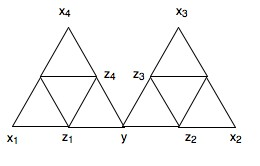
\includegraphics[width=3in]{SW1.jpg} 
   \caption{A subgraph of $ \mathbb{G}_n $. $ y \in \mathbb{G}_{n-1} $ and its neighbours $ x_1,\dots , x_4 \in  \mathbb{G} _{n-1}$.  These 5 points and the remaining 6 nodes are all in $ \mathbb{G}_n $.}
   \label{SW1}
\end{figure}

Let $ (Y_k^{(n)})_{k\geq 0} $ be the simple random walk [SRW] on $ \mathbb{G}_n $.  Unless otherwise indicated, $ Y ^{(n)}_0  = a_0 = 0$, see Figure~\ref{prefrac}.

In Figure~\ref{SW1}
\[ 
P (Y ^{(n)}_{k+1}  = z_i \mid Y ^{(n)}_k) = y) = \frac{1}{4}, \quad 
P (Y ^{(n-1)}_{k+1}  = x_i \mid Y ^{(n-1)}_k) = y) = \frac{1}{4}.
\]

\medskip 

  Let $ 0=T_0, T_1, T_2 ,\dots $ denote successive disjoint%
\footnote{That is, $ Y_{T_{i+1}}^{(n)} \neq Y_{T_{i }}^{(n)}$.}
 hits by $ Y_k^{(n)} $ on $ \mathbb{G}_{n-1} $.
  Then by symmetry, restricting $  Y ^{(n)}_k $ to successive hits on $ \mathbb{G}_{n-1} $, we get 
 \[
 Y^{(n)}_{T_k}  \overset{d}{= }  Y^{(n-1)}_{k}  \quad k\geq 0.
 \]
That is, the restricted SRW on the left is a representative of the SRW on the right.

Fixing $ n $ and restricting to $ m < n  $ we get  a sequence of nested SRW's on $ \mathbb{G}_m $ for each $ m \leq n $.   
  Moreover, we can similarly nest $ Y^{(n)} $ in $ Y^{(n+1)} $ by building in a sequence of independent excursions between $ Y^{(n)}_k $ and $ Y^{(n)}_{k+1} $.%
  \footnote{Note the following.  In Figure~\ref{SW2} the path for $ Y^{(1)} $ is $ a_0a_3a_4a_5 a_6a_2 $ but its extension $  Y^{(2)} $  goes outside the 1-cell determined by $ a_3 a_4 $ in its journey from  $ a_3 $ to $ a_4 $.
  However, it \emph{cannot} in its journey from $ a_3 $ to $ a_4 $ go outside the \emph{two} 1-cells containing $ a_3 $.
  
  Note also that the crossing time of $  Y^{(2)} $ from $ a_3 $ to $ a_4 $ is the same as if it were restricted to the 1-cell $ a_3a_1a_4 $.  This follows from a simple reflection argument at the point $ a_3$.}
 (See \cite{Bar1}*{p15} for a brief discussion and the fact that this can also  be done by using the Kolmogorov extension theorem.)  In this manner we get a prob space $ (\Omega, \mathcal{F}, \mathbb{P} ) $ and random variables $ (Y^{(n)}_k)_{k\geq 0} $ for $ n\geq 0 $ s.t.
  \begin{enumerate}
\item  $ (Y^{(n)}_k)_{k\geq 0}$ is a  SRW on $ \mathbb{G} _n $ beginning at $ a_0 =0 $,
  \item  If $ m< n $ and $ 0=T_0^{m,n} , T_1^{m,n}, T_2^{m,n} , \dots $ are successive disjoint hits by $ (Y^{(n)}_i)_{i\geq 0} $ on $ \mathbb{G}_m $, then 
\begin{equation} \label{sp} 
    Y^{(n)}_{T_k^{m,n}} = Y^{(m)}_{k}  \quad k\geq 0,
\end{equation} 
with equality \emph{everywhere}, not just in distribution.
\end{enumerate}

\emph{Note}
\begin{enumerate}

\item The right side of \eqref{sp} is independent of $ n >m$.
\item  For $   T_k^{m,n} \leq i \leq   T_{k+1}^{m,n} $ ,   $ |Y^{(n)}_i - Y^{(m)}_k| \leq 2^{-m} $, since $ Y^{(n)}_i $ is in the union of the two $ m $-cells containing $ Y^{(m)}_k $.
\end{enumerate} 





\begin{figure}[htbp] %  figure placement: here, top, bottom, or page
   \centering
   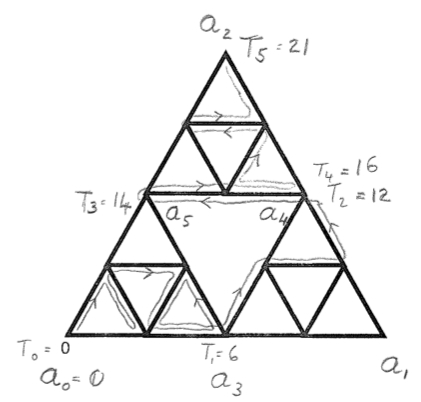
\includegraphics[width=4in]{SW2.jpg} 
   \caption{A sample path for $ (Y^{(2)}_k)_{k\geq 0} $ on $ \mathbb{G}_2 $,  and the nested walks $ (Y^{(1)}_k)_{k\geq 0} $ on $ \mathbb{G}_1 $ and $ (Y^{(0)}_k)_{k\geq 0} $ on $ \mathbb{G}_0 $.}
   \label{SW2}
\end{figure}

\textbf{Example}: In Figure~\ref{SW2} we show a sample path for $ (Y^{(2)}_k)_{k\geq 0} $ on $ \mathbb{G}_2 $.  The \emph{successive disjoint hits} on $ \mathbb{G}_1 $ are at times 
\begin{align*}
&T_0 = T^{2,1}_0 = 0,      & &T_1 = T^{2,1}_1 = 6,  & &T_2 = T^{2,1}_2 = 12, \\
&T_3 = T^{2,1}_3 = 14,      & &T_4 = T^{2,1}_4 = 16,  & &T_5 = T^{2,1}_5 =  21. 
\end{align*}
The induced nested process  $ (Y^{(1)}_k)_{k\geq 0} $ on $ \mathbb{G}_1 $ is
\begin{align*} 
&Y^{(1)}_0 = Y^{(2)}_0 = a_0, &&  Y^{(1)}_1 = Y^{(2)}_6 = a_3, && Y^{(1)}_2 = Y^{(2)}_{12}= a_4 \\
&Y^{(1)}_3 = Y^{(2)}_{14} = a_5, &&  Y^{(1)}_4 = Y^{(2)}_{16} = a_4, && Y^{(1)}_5 = Y^{(2)}_{21}= a_2.
\end{align*}  

The  \emph{successive disjoint hits} of $ (Y^{(2)}_k)_{k\geq 0} $ and $ (Y^{(1)}_k)_{k\geq 0} $  on $ \mathbb{G}_0 $ are at times 
\[
 T^{2,0}_0 =  T^{1,0}_0 = 0, \qquad  T^{2,0}_1 =  21, \qquad T^{1,0}_1 = 5.
 \]
The induced nested process  $ (Y^{(0)}_k)_{k\geq 0} $ on $ \mathbb{G}_0 $ is
\[
Y^{(0)}_0 = Y^{(1)}_0 = Y^{(2)}_0 = a_0, \qquad Y^{(0)}_1 = Y^{(1)}_{5} = Y^{(2)}_{21} = a_2.
\]

\begin{figure}[htbp] %  figure placement: here, top, bottom, or page
   \centering
   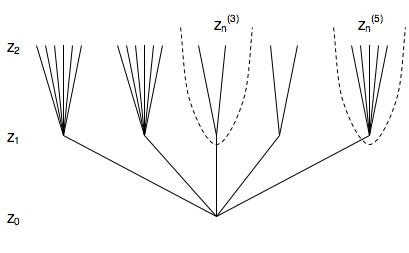
\includegraphics[width=4in]{SW3.jpg} 
   \caption{Crossing time branching process and sub processes.}
   \label{SW3}
\end{figure}

(See Figures~\ref{SW2},  \ref{SW3} and Section~\ref{secbp}.) The \emph{branching process} of crossing times $ Z_n $ for $ Y^{(n)} $  from $ 0 = a_0 $ to $ \{a_1,a_2\} $ here has values
\[  Z_0 = 1, \quad Z_1 = 5, \quad Z_2 = 21.\]
The branching (sub-) processes $ Z_n^{(i)} $ of crossing times between  the $ i\!-\!1$th and $ i $th successive hit for $ Y^{(n)} $ on $ \mathbb{G}_1 $ have values 
\begin{align*}
& Z_1^{(1)} = 1, &&  Z_1^{(2)} = 1, &&  Z_1^{(3)} = 1, &&  Z_1^{(4)} = 1, && Z_1^{(5)} = 1, \\
&   Z_2^{(1)} = 6, &&  Z_2^{(2)} = 6, &&  Z_2^{(3)} = 2, &&  Z_2^{(4)} = 2, && Z_2^{(5)} =5.
\end{align*} 






%%%%%%%%%%%%%%%%%%%%%%%%%%
\subsection{The branching process $ Z_n $}\label{secbp}
Let $ Z_n $ be the crossing time for $ (Y^{(1)}_k)_{k\geq 0 } $ from $ 0 = a_0 $ to $ \{a_1,a_2\} $ in Figures~\ref{prefrac} and \ref{SW1}.
Let $ \tau = Z_1 \ (= T_1^{0,1}) $. 
 
 Then by construction $ (Z_n)_{n\geq 0} $ is a simple branching process with 
\begin{equation} \label{}
Z_0 = 1, \quad Z_{n+1} = \sum_{i=1}^{Z_n}Z_{1,i} =  \sum_{j=1}^{Z_1}Z_{n,j},
\end{equation} 
with iid  $Z_{1,i}   \overset{d}{=} \tau $ giving the offspring distribution and iid $ Z_{n,j}
 \overset{d}{=} Z_n$.
 
 The first equality is clear and the second is obtained by taking the $ Z_1 $ trees rooted at level one.

 

%%%%%%%%%%%%%%%%%%%%%%%%%%%%%%%%%%
\subsection{The p.g.f. for $ Z_n $}
 In order to investigate $ Z_n $ it is natural to find its \emph{probability generating function} [p.g.f.].%
\footnote{\emph{Properties of a  p.g.f.}: (see \cite{Lal}).  If $ Z$ is a non negative integer valued R.V.\ then its p.g.f.\ is defined by
\[  f(s) = \sum_{k\geq 0}  P(Z=k)s^k = \mathbb{E} (s^ Z).\]
The power series for $ f $ converges absolutely for $ |s | < 1 $, and the coefficients contain all the probabilities needed to describe $ Z$.

Clearly,
\begin{align*}
f'(s) &= \sum_{k\geq 0}  kP(Z=k)s^{k-1} = \mathbb{E} \big( Zs^{ Z -1} \big),\\
f''(s) &= \sum_{k\geq 0}  k(k-1)P(Z=k)s^{k-2} = \mathbb{E} \big(Z(Z-1)s^{ Z-2} \big).
\end{align*}


All moments can be computed from the derivatives of $ f  $ at $ 1 $.  In particular,
\[
f(1) = 1, \quad f'(1) = \mathbb{E} (Z ) , \quad f''(1) = \mathbb{E} (Z ^2) - \mathbb{E} ( Z ),
\]
and so 
\[
 \text{Var}\, Z = \mathbb{E} \big( Z - \mathbb{E}   Z \big)^2 
     = f''(1) - f'(1) - \big(f'(1)\big)^2.
     \]
}
Consider first  $ \tau =Z_1$:
\begin{equation} \label{} 
f(s) := \mathbb{E} (s^\tau) = \sum_{k\geq 0} P(\tau = k) s^k .
\end{equation} 
To compute this, let  
\begin{align*}
f_c(s) &= \mathbb{E} ^c(s^\tau) \quad \text{where $ c $ is the midpoint of $ 0a_1 $ or $ 0a_2 $},\\
f_b(s) &= \mathbb{E} ^b (s^\tau) \quad \text{where $ b $ is the midpoint of $  a_1 a_2 $}.
\end{align*}
Then it is easy to see from Figure~\ref{prefrac} that 
\begin{align*}
f(s) &= s f_c(s) \\
f_c(s) &= \frac{1}{4} s (f(s) + f_c(s) + f_b(s) + 1)\\
f_b(s) &= \frac{1}{2} (f_c(s) + 1).
\end{align*} 
Solving,
\begin{equation} \label{pgf1} 
f(s) = s^2/(4-3s), \quad \mathbb{E} \tau = f'(1) = 5, \quad \mathbb{E} \tau^k < \infty \ \forall k. 
\end{equation} 


\medskip More generally, let 
\[ f_n(s) =   \mathbb{E} s^{Z_n} = \sum_{k\geq 0}  P(Z_n=k)s^k   .\]
Then
\begin{equation} \label{} 
f_0(s) = s, \quad f_1(s) = f(s) = \frac{s^2}{4-3s}, \quad f_n(s) = \overset{1}{f}\circ \dots \circ \overset{n}{f}(s).
\end{equation} 
The first is immediate since $ Z_0=1 $ and the second is from \eqref{pgf1}.  The third is a standard branching process / p.g.f.\  argument using either the fact that $ Z_{n+1} $ is $ Z_n $ iid copies of $ \tau \overset{d}{=} Z_1 $, or is $ Z_1 $ iid copies of $ Z_n $ (consider the trees rooted at level one).% 
\footnote{More  precisely
\begin{align*}
f_{n+1}(s) &= \mathbb{E} s^{ Z_{n+1} } 
 = \mathbb{E} s^{ \sum_{i=1}^{ Z_1 }  Z_{n,i} } \quad \text{for iid }  Z_{n,i} 
                    \overset{d}{=} Z_n \\
  &=\mathbb{E}   \prod_{i=1}^{ Z_1 } s^{  Z_{n,i} }  
  = \mathbb{E} f_n(s)^{ Z_1 } \quad \text{since }\mathbb{E} s^{  Z_{n,i} }  = f_n(s) \\
  &= f ( f_n(s)).
\end{align*}
\emph{Or}
\begin{align*}
f_{n+1}(s) &= \mathbb{E} s^{ Z_{n+1} } = 
 \mathbb{E} s^{ \sum_{j=1}^{   Z_n }  Z_{1,j} } \quad \text{for iid }  Z_{1,j} 
                    \overset{d}{=} Z_1 \\
&= \sum_{k\geq 0} P(Z_n = k) \mathbb{E} s^{ \sum_{j=1}^{ k }  Z_{1,j} } 
=  \sum_{k\geq 0} P(Z_n = k)  f(s)^k\\
&= \mathbb{E} f(s)^{Z_n} = f_n(f(s)).
\end{align*} 
}



%%%%%%%%%%%%%%%%%%%%%
\subsection{Rescaled process $ W_n $ and its limit }
Since 
\[
Z_{n+1} =  \sum_{i=1}^{ Z_n }  Z_{1,i}   \quad \text{for iid }  Z_{1,i} 
                    \overset{d}{=} Z_1,  
\]
it follows 
\[
\mathbb{E}( Z_{n+1} \mid Z_n ) =( \mathbb{E} Z_1)\, Z_n = 
5 Z_n
\]
Let $ W_n = Z_n/5^n $.  Then 
\[  \mathbb{E} ( W_{n+1} \mid  W_n) =  W_n, \quad 
   \mathbb{E} \mathbb{W_1}^2 < \infty,
   \]
   and so by martingale theory, see \cite{Har},% 
   \footnote{*** Include some info on branching processes and this result} 
\begin{equation} \label{}
Z_n/5^n =  W_n \to W \text{ a.s.},
\end{equation} 
where $ 0 < W < \infty $ a.s.  

 In particular, the growth rate of $ Z_n $ is of order $ 5^n $.
 
%%%%%%%%%%%%%%%%%%%%%%%%%%%%%%%%%%%%%%%%%%%%%%%
%%%%%%%%%%%%%%%%%%%%%%%%%%%%%%%%%%%%%%%%%%%%%%%%%%
%%%%%%%%%%%%%%%%%%%%%%%%%%%%%%%%%%%%%%%%%%%%%%%
\subsection{Subtrees $ Z_n^{(i)} $ of $Z_n $}   
The process $ Z_n $ gives the number of steps required for $ Y^{(n)} $   to cross $ \mathbb{G}_0 $.  After dividing by $ 5^{-n} $ we get a.s.\ convergence to a (continuous) positive finite distribution $ W $.

\emph{Fix} $ m $ and consider those $ n \geq m $. 
Let $   Z_{n,m}^{(i)} $ denote the number of steps taken by   $ Y^{(n)} $between hit $ i-1 $ and hit $ i  $ on $ \mathbb{G}_m $.   That is
\begin{equation} \label{eq1}
 Z_{n,m}^{(i)} =T^{n,m}_i - T^{n,m}_{i -1}. 
\end{equation} 
These are independent for fixed $ n $ and $ m $, and on normalising we get
\begin{equation} \label{eq2}
 W^{(i)}_m := 5^{-n}  Z_{n,m}^{(i)}  \to W_m^{(i)} \text{ (say) }    \overset{d }{=} 5^{-m} W,\text{ a.s.\ as } n\to \infty,
\end{equation} 
where for each $ m $ the $ W^{(i)}_m $ are independent.




%%%%%%%%%%%%%%%%%%%%%%%%%%%%%%%%%%%%%%%%%%%%%%%
%%%%%%%%%%%%%%%%%%%%%%%%%%%%%%%%%%%%%%%%%%%%%%%%%%
%%%%%%%%%%%%%%%%%%%%%%%%%%%%%%%%%%%%%%%%%%%%%%%
\section{\textbf{Construction of Diffusion Process on SG(2)}}\label{seccp}
Let
\begin{equation} \label{}
X_t^n = Y^{(n)}_{[5^nt]} \quad t \geq 0,
\end{equation}
where ``$ [\cdot] $ '' is the ``integer part of''.  This is the natural time scaling.

\begin{theorem}
 The process $ X^n_t $ converges a.s.\ and uniformly on compact intervals to a continuous process $ (X_t)_{t\geq 0} \in G$.
\end{theorem}

\begin{proof}[Proof Outline]  Fix $ m \geq 0$ and $ i\geq 0 $.

Suppose 
\[   \sum_{j=1}^i W_j^{(m)} < t < \sum_{j=1}^{i+1}W_j^{(m)} \]
(The idea is that $ t $ will be in the time interval between successive hits $ i $ and $ i+1 $ on $ \mathbb{G}_m $ of the limit process $ X_t $.)

Then from \eqref{eq1} and \eqref{eq2} for $ n \geq n_0 (\omega)$, say, 
\[   5^{-n} T_i^{m,n} < t < 5^{-n} T_{i+1}^{m,n} .\]
It follows from Note(2) following \eqref{sp}  that 
\[ |X_t^n - X_t^{n'}| \leq 2^{-m+1}  \]
for $ n,n'\geq n_0 $.

Thus $X_t^n $ is Cauchy in $ n $ and so converges a.s.\ for each $  t$.

The fact convergence is uniform on compact intervals and the limit is continuous is by a similar argument.
See \cite{Bar1} for details.
\end{proof}



%%%%%%%%%%%%%%%%%%%%%%%%%%%%%%%%%%%%%%%%%%%%%%%
%%%%%%%%%%%%%%%%%%%%%%%%%%%%%%%%%%%%%%%%%%%%%%%%%%
%%%%%%%%%%%%%%%%%%%%%%%%%%%%%%%%%%%%%%%%%%%%%%%
\section{\textbf{Properties  of Diffusion Process on SG(2)}}
\begin{theorem}\mbox{}
 \begin{enumerate}

\item  There exists a continuous strong Markov%
\footnote{See \cite{Lam}*{Chapter 9}.) The strong Markov property is that a.s.
\[  P^x(X_{\tau + t} \in D \mid \mathcal{F} _\tau) = P^{X_\tau}(X_t \in D ) ,\]
for any stopping time $ \tau $ and associated $ \sigma $-algebra $ \mathcal{F}  _\tau $.}
process $ X = (X_t, t\geq 0, P^x, x \in G ) $ on $ G $.

\item The semigroup on $ \mathcal{C} (G) $ defined by
\[ P_tf(x) = \mathbb{E} f(X_t) \]
is Feller%
\footnote{That is, $ P_t f $ i continuous if $ f $ is continuous.}
and is $ \mu_G $ symmetric:
\[  \int_G f\, P_t g \, d\mu_G =  \int_G P_tf\,  g \, d\mu_G.\]

\item $ X $ is locally isotropic%
\footnote{If $ \phi:A\to B $  and $ \phi : \partial A \to \partial B $ are isometries  where $ A,B \subset G $, then 
\[ \forall x \in A \ \forall E \subset A \quad P^x( X_{t \wedge T_{\partial A}}\in E,\  t\geq 0)
=  P^{\phi(x)} ( X_{t \wedge T_{\partial B}}\in \phi(E),\  t\geq 0).
\]
Here $t \wedge T_{\partial A}  $ is the minimum of the time $ t $   and the time $  T_{\partial A} $ of first reaching the boundary $ \partial A $. Similarly for $t \wedge T_{\partial B} $.
}
 w.r.t.\ the metric $ _G $ and the Euclidean metric.

\item Let $ (T^n_i)_{i\geq 0} $ denote successive disjoint hits by $ X_t $ on $ \mathbb{G}_n $.  Then 
$ \widehat{Y}_i^{(n)} := X_{T^n_i} $  defines a SRW on $ \mathbb{G}_n  $. Moreover, $ \widehat{Y}_{[5^n t]}^{(n)} \to X_t $ uniformly on compact sets a.s.

In particular, $ X_t $ is the process in Section~\ref{seccp}.
\end{enumerate} 

\begin{proof} See \cite{Bar1}*{Sections 6,7}. The main point is to prove (1).   \end{proof}


 




\end{theorem} 
%%%%%%%%%%%%%%%%%%%%%%%%%%%%%%%%%%%%%%
%%%%%%%%%%%%%%%%%%%%%%%%%%%%%%%%%%%%
%%%%%%%%%%%%%%%%%%%%%%%%%%%%%%%%%%%%%%%%%%
\begin{thebibliography}{9} 



\bib{Bar1}{article}{
   author={Barlow, Martin T.},
   title={Diffusions on fractals},
   conference={
      title={Lectures on probability theory and statistics},
      address={Saint-Flour},
      date={1995},
   },
   book={
      series={Lecture Notes in Math.},
      volume={1690},
      publisher={Springer},
      place={Berlin},
   },
   date={1998},
   pages={1--121},
%   review={\MR{1668115 (2000a:60148)}},
}


\bib{Har}{book}{
   author={Harris, Theodore E.},
   title={The theory of branching processes},
   series={Die Grundlehren der Mathematischen Wissenschaften, Bd. 119},
   publisher={Springer-Verlag},
%   place={Berlin},
   date={1963},
   pages={xiv+230},
%   review={\MR{0163361 (29 \#664)}},
}
	

\bib{Lal}{article}{
   author={Lalley, Steven},
   title={Generating function methods},
   note={lecture course notes},
   date={2007},
   eprint={galton.uchicago.edu/~lalley/Courses/313/GeneratingFunctions.pdf}, 
 }
   
  
\bib{Lam}{book}{
   author={Lamperti, John},
   title={Stochastic processes},
   note={A survey of the mathematical theory;
   Applied Mathematical Sciences, Vol. 23},
   publisher={Springer-Verlag},
%   place={New York},
   date={1977},
   pages={xvi+266},
%   review={\MR{0461600 (57 \#1585)}},
}




\end{thebibliography}





\end{document}


